\section{Introduction}

What is linux filesystem api?
Why is it important
How many years it has been ParComputind
How it's learned today
Is an api older than the internet still documented well on qa websites
study shows that stackoverflow is the most visited
Others show its dymanics on recent API

Important when writing character device drivers or any other device driver[https://www.tldp.org/LDP/lkmpg/2.4/html/x579.html]
[https://www.nxp.com/files-static/soft_dev_tools/doc/ref_manual/Linux%20Device%20Drivers.pdf]
documentation is hard to understand [ref]
Additionally, many POSIX functions share similar names, while others have different flags that change their behavior[example]
Explain coverage
posix has known problems
this study complains about it and its security issues
Many blog posts alsocomplain about its usage
This is a way to quantify this stuff
'
Robillard study the decisions open source developers make while creating
developer documentation for frameworks and libraries [9]
s. They concluded that the community answers review, conceptual,
and how-to questions more frequently than any other type, with review questions
achieving a 92\% accepted answer rate [21]. Posnett et al. studied the nature of expertise
among Stack Exchange participants and found that participation in online Q/A sites
does not necessarily lead to increased expertise as measured by peer scoring [16]
Parnin and Treude study availability of documentation
across APIs within StackOverflow and find that it is very uneven, some APIs are well
covered, while others receive very little attention [20]. Jiau and Yang address this concern
and assert that more obscure API components benefit from a trickle down affect of
similar API components [11].
The work most similar to ours is recent work by Parnin et al. who also evaluated
the degree to which specific APIs are discussed within the community [15].
'
Theory?
Model with types

\begin{itemize}
  \item
  RQ1 Can we rely on the Stack Overflow crowd to discuss all of Linux kernel filesystem APIs?
  \begin{itemize}
    \item
    RQ1.1 Are the API methods widely covered?
    \item
    RQ1.2 Is there a relationship between number of discussions around a function and its usage in Github repositories?
    \item
    RQ1.3 Are there still ongoing discussions about these APIs? How fast are they covered?
  \end{itemize}
  \item
  RQ2 What kind of questions are asked about the APIs?
  \begin{itemize}
    \item
    RQ2.1 What are the most common keywords that appear in questions?
    \item
    RQ2.2 How often do pairs of components appear together in questions?
  \end{itemize}
  \item
\end{itemize}
RQ2.2 tries to understand how different functions are used and asked for together. This could be used to build models...
To verify that the data follows the general trend of [ref]

Contribution:
- Reproduces the results of earlier studies on different datasets
- Analyzes Questions that mention two or more functions in an attempt to show which two questions are confused together or asked about together

Understanding quantitative qualities about questions and linking them to qualitative ones can help build models that depend on theat sort of questions.

%TODO Check for consstency

\section{Data and Methodology}
Research questions?
data:
Filesystem API : scraped function, structure names and the categories they fall into from the official docs [refs], then verified by hand. The documentation is wellformatted, so it was easy to get header names and using a script written in jquery javascript. The result was loaded to a database, and each function was given a unique id and assigned to a category.
The API functions are mostly not changed between versions [ref], but we used the ones from 4.16.0

Stack Overflow: StackOverflow provides data dumps, under a Creative Commons license on archive.org every three onths along with the other stackexchange websites. downloaded a database dump (dates to 12/2017), loaded on a database. due to the huge size of data (42 Gb in total), posts were filtered by tags (mention here), then all the answeres related to them were added. All stackoverflow posts are required to be tagged, and most tagged posts contain the language in qustion so it was ok to filter. Tags are mentioned in text inside the posts table, and not in a separate table as in the data explorer [ref]. so To improve the performance of the data filtereing, the tags column was added to a fulltext index [ref]. this resulted in an order of magnitude increase in performance (several minutes instead of several hours when using like search) over a slight decrease in accuracy.
Linking: To gather our data, we used a process adopted from Parnin [15].
In our case, a link is a connection between a StackOverflow question and a Linux filesystem function. There are word links which occur in words, url links in urls, code links in <code> tags and code block links inside <pre> code blocks.
Found using case-insensitive word boundary search.
search was done on title and body of questions and answers, and each matching question was recorded in the database. We also searched the answers, and each matching answer was reported to belong to the question of the answer. Further queries were made for each RQ, as explained in [section somewhere]
Fulltext was used again to provide faster results (several minutes instead of hours). Fulltext index builds a full index of all the words in the selected fields and ranks them .. % check how it works
 According to the documentation, [ref] it produces no false positives, but might miss some cases for very large texts [ref]
In our case, the size of each question is reasonably small, so we could do that.
% mention the number of matches

Usage Data: The usage data was gathered by doing searching for the filesystem API using Github code search API. The search was done using a script that issuea a search request for each function and record the total number of records as reported by the response The search was limited to files written in c only to prevent any similar named stuff from other languages from affecting the data.
with a random wait time between 3-10 seconds to circumvent the rate-limiting on the server.
Github code search doesn't include forked repositories unless the forked repository has more stars than the original repo.
% TODO define thread
Frequency analysis: to answer RQ2, we did a basic frequency analysis on the threads.
Question texts were sanitized by removing all html tags.
We did not consider code samples, as they are irrelevant to what the question asks
We tokenized the texts by word boundary
Then stemmed them using porter stemmer [ref]
Then filtered out words considred stop words. We used the list of default stop words in the English language, and included other stop words common in stackoverflow conversations like "code", "please", "thanks". The full list is available in the git repo below.
After that, we fed the single words, bigrams and trigrams to a frequency counter.
We did this for questions alone, and for answers.

Reproducibility:
All our data are provided publically on github. Contains scripts, queries and result csv files.
https://github.com/zalsader/LinuxFSQuestions

\section{Results}
\subsection{Data Reliability}
we examin RQ1...
\subsubsection{Coverage}
RQ1.1
Are they widely covered
look for functions
Coverage is the percentage of the API elements that have at least n threads discussing
the class, where n is called the saturation level
Report on coverage by multiple n. % TODO table?
\begin{figure}
  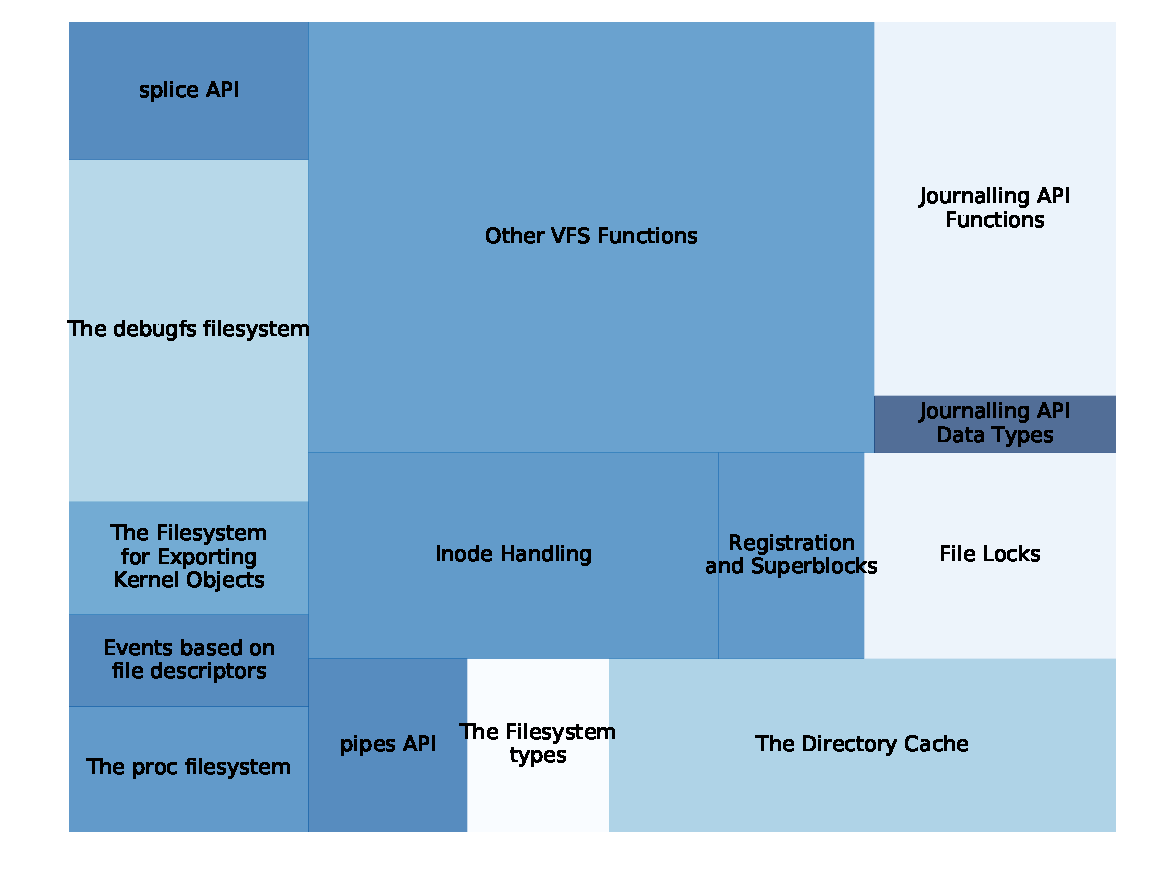
\includegraphics{scripts/figures/1-1-coveragebycategory.pdf}
  \caption{Coverage by category}
  \label{fig:covbycategory}
\end{figure}

We also examined the coverage per category, and the results are in figure
Although old, the api is not yet widely covered
but enough to continue our analysis
Number of threads? %TODO
RQ1.2
Are they related to the usage
We mined the usage date from github using thescript.
Results are plotted in the graph on a log-log scale
We fount that we have a slope of 0.51 and regression of? %TODO
A Spearman’s rank correlation coefficient?
which translates into a sublinear dependence of y on x
On the average, the demand for class documentation from SO grows slower
than class usage in the code. as past studies found


\begin{figure}
  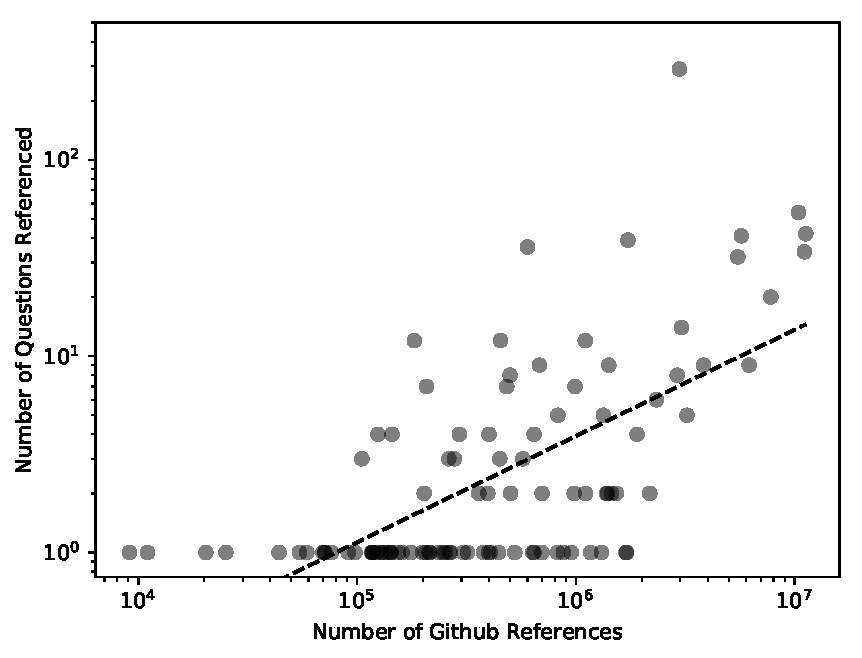
\includegraphics{scripts/figures/1-2-usage-vs-coverage}
  \caption{Usage vs number of references on a log-log scale}
  \label{fig:usageref}
\end{figure}

RQ1.3
Coverage over time
Coverage is increasing steadily over time
It is interesting to see that the coverage is still growing steadily even after 30 years from the API
This means that there are still questions to be asked about the API and the documentation available is still not enough

\begin{figure}
  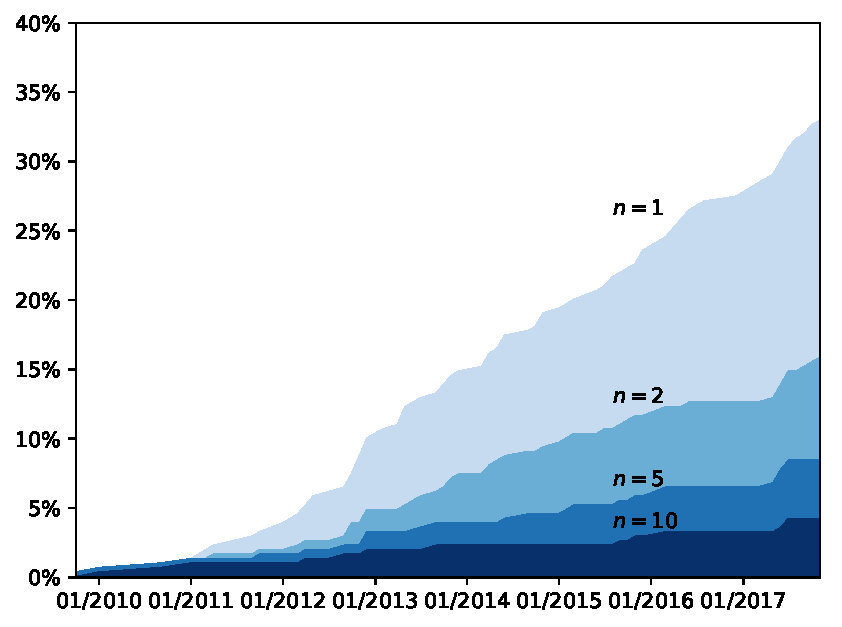
\includegraphics{scripts/figures/1-3-coverage-by-time}
  \caption{The coverage for the API over time}
  \label{fig:coveragetime}
\end{figure}


RQ2
Questions asked about the API
RQ2.1
To answer this question, we identify the keywords most common in questions and answers that contain any of the linux filesystem API functions and structures, excluding code samples as defined in section[ref]. Since the words are stemmed using the porter stemmer, many of the terms in the figure appear to be misspelled or incomplete.
From the single word results, it seems that most questions ask about how to `use' the functions, how they `work', and some also ask for `examples'. Since we are asking questions about the filesystem API, the words `write', `read' and `kernel' appeared very often. In addition, a lot of questions reported `problems' or asked for `solutions'. The results from mining answers for single word frequency do not seem very different.

The results for bigrams and trigrams seem to result in more interesting terms, after the most common `kernel module' and `linux kernel module', many questions contained `device driver', `block device' and `linux device driver' in reference to questions about vfs functions related to device drivers, like this post [https://stackoverflow.com/questions/11578504/how-sys-open-works]. Additionally, many questions asked for a `better way', or the `best way' to achieve a task.
The results from mining bigrams and trigrams of answers are very similar, with the difference that `better way', `best way' and `create new' appear more often than other terms.
%caveat: skewed by large coverage

\begin{figure}
  \begin{subfigure}
    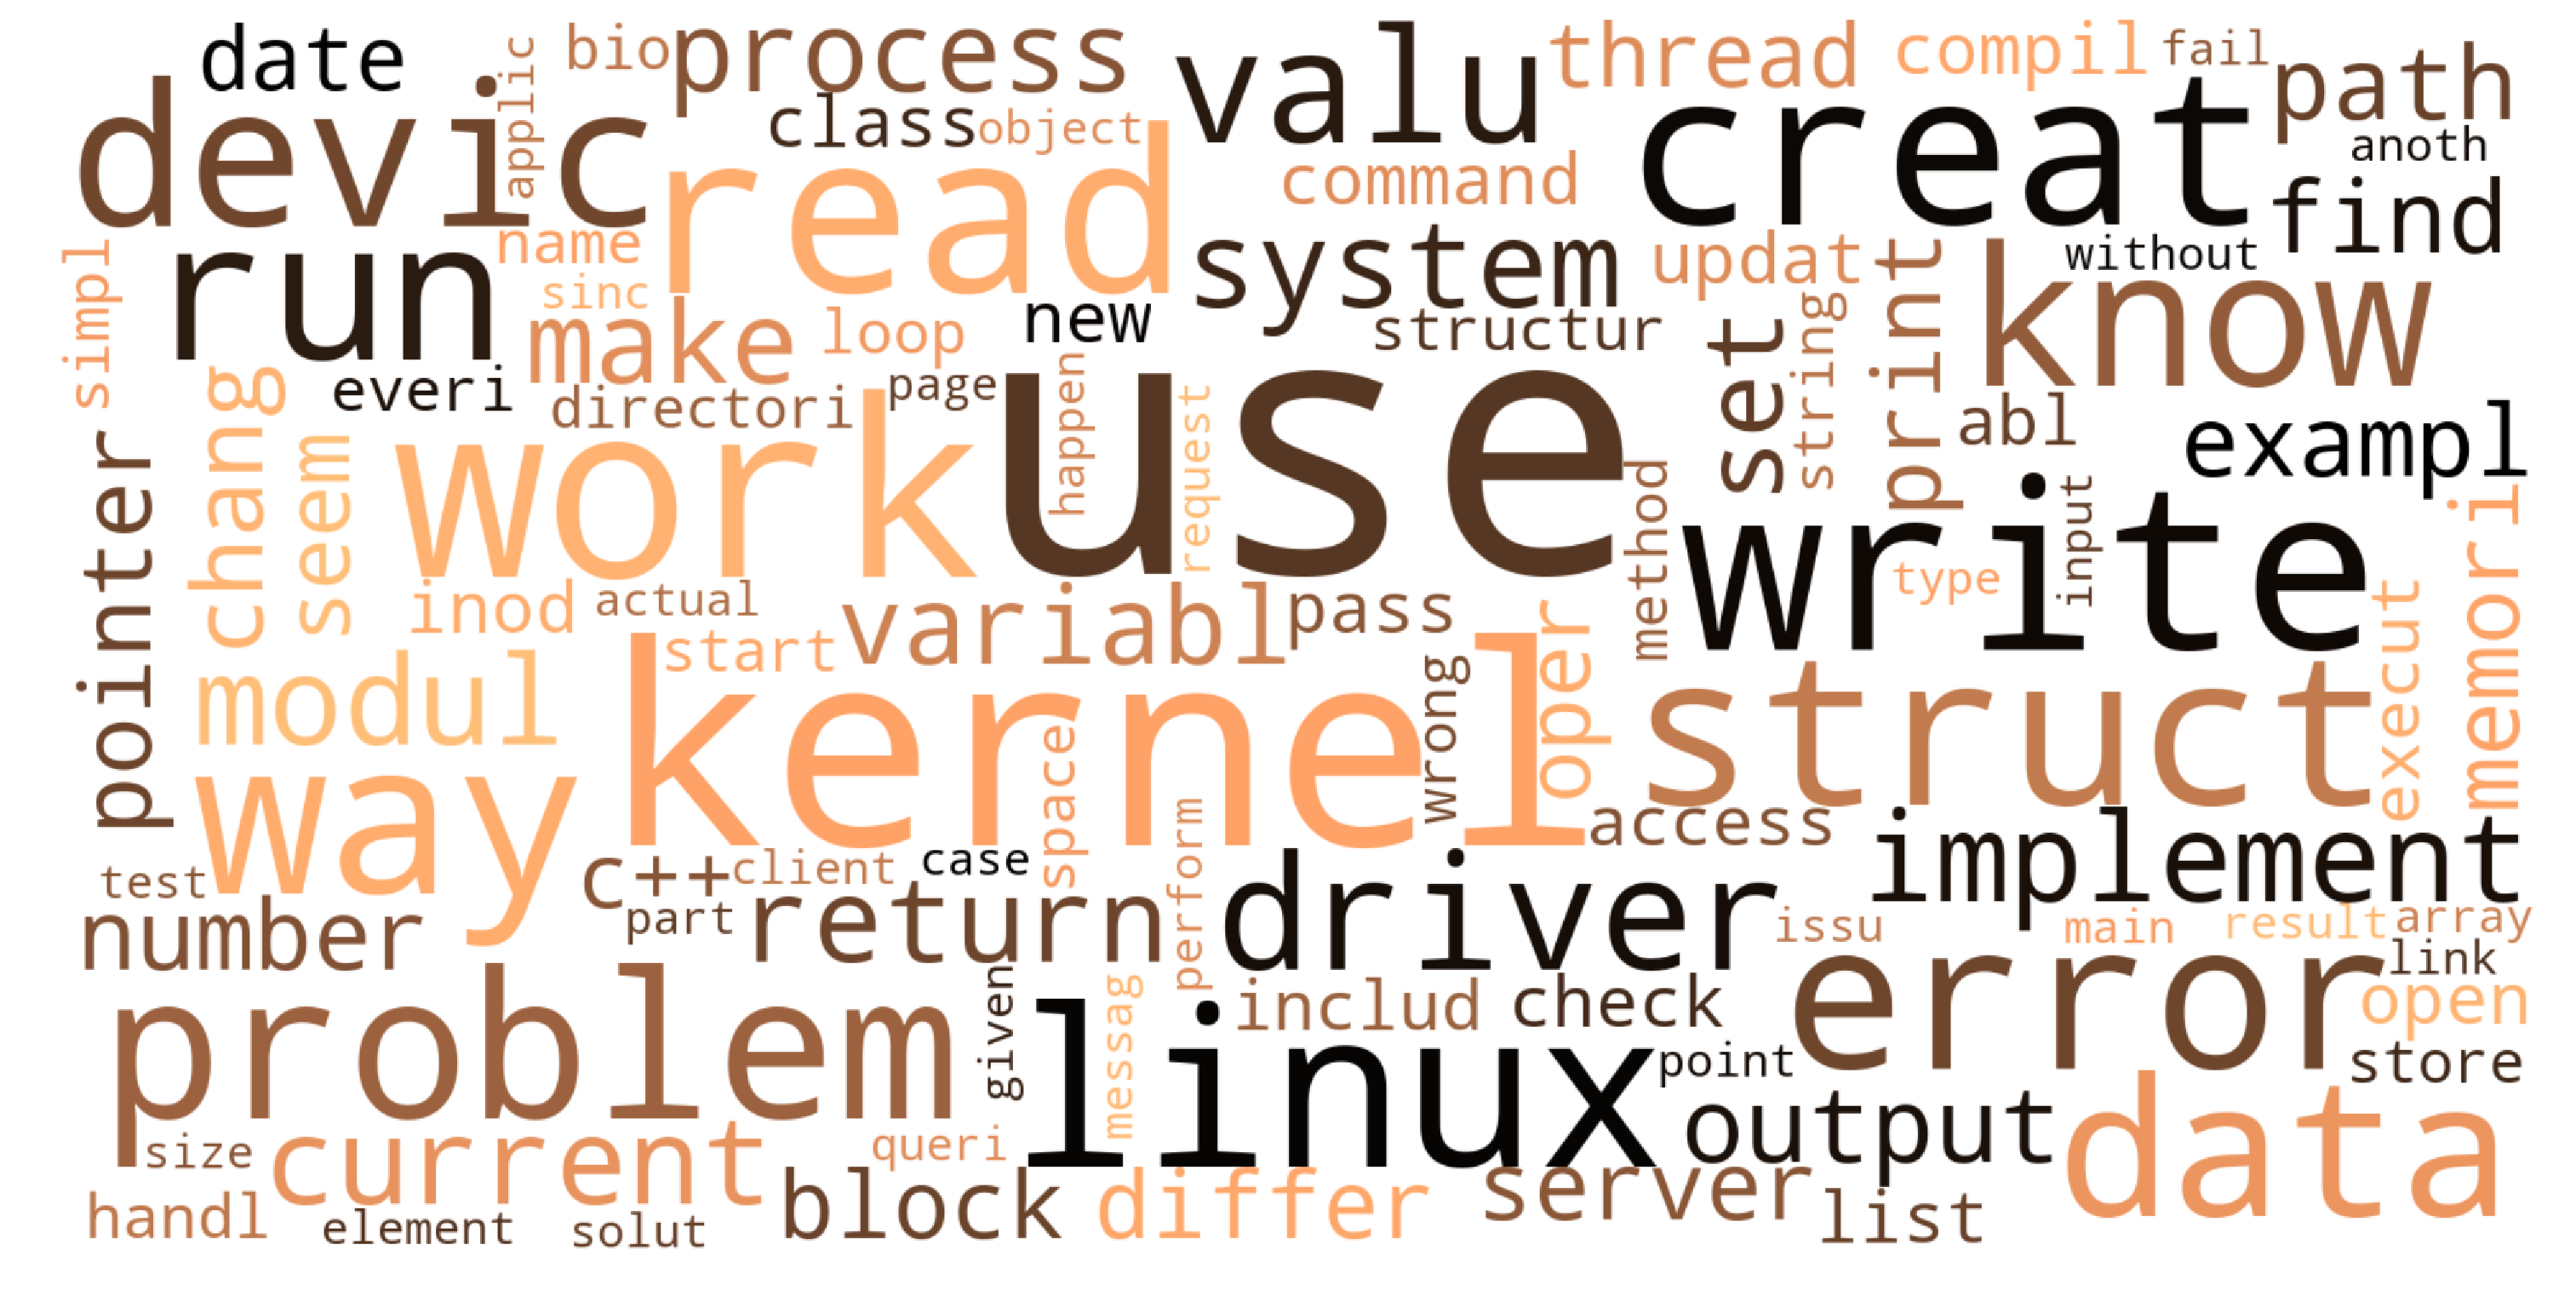
\includegraphics{scripts/figures/2-0-1-allquestions.pdf}
  \end{subfigure}%
  \begin{subfigure}
    
\includegraphics{scripts/figures/2-0-2-allquestions.pdf}
  \end{subfigure}%
  \caption{Word clouds generated by the most common words in all matching questions using single words (a) and bigrams (b)}
  \label{fig:wcall}
\end{figure}

RQ2.2
Common functions together
This questions explores how often do questions ask about more than one function or API. This peeks into the question of confusion. To do that, we searched the recorded results from [ref] for questions that contain two or more API functions. The table[] shows the functions that appear together the most within the same category, and table [] shows how much appears for different categories. From the results we can see that, within the same category, sequential file processing methods \texttt{seq_*} are very commonly asked about together within the same question. This is because they are commonly used together to build device drivers, and many questions provide examples on how to use them, see this question [https://stackoverflow.com/questions/17663692/file-operations-in-drivers].
Additionally, \texttt{debugfs_create_dir} and \texttt{debugfs_create_file} are commonly found togetherm since both of them can be used to create directories. The difference between them is that the former is the recommended function to create directories in debugfs, while the latter can be used to create directories and files alike. Most answers that reference both function explain this difference, including this one [https://stackoverflow.com/questions/42235800/write-to-debugfs-from-linux-kernel-module]
debugfs [https://www.kernel.org/doc/Documentation/filesystems/debugfs.txt] is a simple-to-use RAM-based file system commonly used for debugging. For that reason, we can find many questions that contain examples for using \texttt{debugfs_*} functions.

%TODO include tables

summary

Threats to validity
Generalizability:  RQ1 generalizes findings of previus work in java api domain into the linux filesystem API domain, but it is still not known if this generalizes to other domains.
stackoverflow stuff
The remaining threats listed below arise from the fact that StackOverflow is unstructured
natural language text, and extracting information therefrom is naturally a noisy
process.
However, a mention of a class in an SO question or answer does not necessarily mean
that the message is about that class; but it does mean that the message is relevant somehow
to the class.
splitting
similar names
incorrect tags or formatting: often fixed by moderators.
Github only includes opensource projects in its search, which means that the usage data we derived is biased towards opensource projects. Github allows any user to fork any repository they want, this is mitigated by the github code search itself, since it does not include any forks that have less stars than the original repositories. there's a possibility of functions sharing the same name, but the function names we considered are unique enough as we concluded from manual inspection of the search results.
word frequency analysis might be biased towards functions that have more questions about them. This was not found to be a major concern in our analysis, but we could explore calculating the word frequency per function or category of functions.

future work
Qualitative study of the questions we found,
which can help produce machine learning models to predict stuff
Include other sources like linux mailing lists and issues in the study.
Expant to other linux kernel functions
We could use the


%TODO maybe search for other keywords with functions?













.
